\section{Background and Related Work}
\label{sect:BACKGRELWORK}

In this section, first we introduce basic features of the MPS platform, and then we discuss other existing projects that aim to add support for general purpose languages into MPS.

\subsection{JetBrains MPS}
\label{sect:MPS}

JetBrains MPS is a complete language workbench --- an integrated development environment that allows developers to create their own languages and use them to write code.
The code can then be transformed into a target language, typically a GPL, such as Java or C, and eventually compiled into executable programs.

As we already indicated, MPS differs from typical IDEs in one important aspect --- the projectional editor.
The developer does not work with the textual representation of the source code directly, but rather with its AST that is the model of the code.
Basically, when using the MPS projectional editor, programs are created by assembling the tree (AST) out of predefined building blocks of selected languages.
The definition of a language in MPS dictates, where in the AST can certain elements be placed and how they can be nested inside other elements.
On the other hand, in traditional IDEs it is the parser that constructs an AST of a program using the language's elements.

The building blocks of MPS models are called nodes.
Code of any program in MPS is built from nodes, which represent instances of concepts defined in one of the languages that the program declares to be using.
In the context of MPS, a concept is, in fact, a building block of a language definition.
We use the terms \emph{MPS concept} and \emph{AST node} when needed to avoid confusion.

One of the key advantages of projectional editing stems from the separation of abstract and concrete syntax.
While AST provides a complete and precise representation of the code, the way it is displayed on the screen and the way the user interacts with it are unconstrained.
The editor can take any visual form and shape.
The language author can define multiple alternative visualizations and let the developer to choose one that fits best the task at hand --- for example, editing, debugging, reviewing, resolving merge conflicts, etc.
In particular, the visual representations are not bound to be just textual at all.
For example, blocks corresponding to branches of an \code{if-then-else} statement can be aligned next to each other and displayed with different background colors.

The definition of an MPS concept (language element) consists of several aspects, where each aspect codifies a different part of the AST nodes' behavior.
The essential aspects are the following: \emph{Structure} (abstract syntax), \emph{Editor} (concrete syntax) and \emph{TextGen}.
Editor defines the concrete syntax (i.e., how the code is visualized and edited) and TextGen specifies how AST nodes are transformed into textual representation.
If, instead of generating text directly, programs in the language are supposed to be transformed into another language that is available in MPS, the Generator aspect must be used to specify the model-to-model transformation rules.
Since only the Structure, Editor and TextGen aspects are relevant for the contribution of this paper, we describe these three below in more detail, and neglect other aspects such as type system and data-flow.

Languages are built from the concepts using techniques known from object-oriented programming --- containment, inheritance, interfaces, and so on.
Therefore, a definition of a whole language in MPS typically has an object-oriented and hierarchical nature.

\paragraph{Structure.}
The fundamental aspect of any MPS language is Structure.
It must be created first for each intended element (concept) of the language.
Structure specifies core attributes of an MPS concept such as the name, inheritance relationships, possible child concepts (including their types and cardinalities), the implemented interfaces, and references to other AST nodes.
% other properties (fields of any type that can hold values), etc.
Figure~\ref{fig:if_statement_structure} shows definition of the Structure aspect for the \code{if} statement.

The definition of Structure restricts the type of AST nodes that can appear at a particular place in the tree.
For example, one can restrict the condition in the \code{if-then-else} statement to be a boolean expression, and the \code{then}-block to be a list of statements.

\begin{figure}[ht]
\centering
\begin{alltt}
\small
\mpskeyword{concept} IfStatement \mpskeyword{extends} Statement
        \mpskeyword{implements} IContainsStatementList
                   IDontSubstituteByDefault
                   IConditional

  \mpskeyword{instance can be root:} false
  \mpskeyword{alias:} \mpsalias{if}
  \mpskeyword{short description:} \mpsplaceholder{<no short description>}

  \mpskeyword{properties:}
  \mpsproperty{forceOneLine}   : boolean
  \mpsproperty{forceMultiLine} : boolean
  
  \mpskeyword{children:}
  \mpsproperty{condition}        : Expression[\mpscardinality{1}]
  \mpsproperty{ifFalseStatement} : Statement[\mpscardinality{0..1}]
  \mpsproperty{ifTrue}           : StatementList[\mpscardinality{1}]
  \mpsproperty{elsifClauses}     : ElsifClause[\mpscardinality{0..n}]
  
  \mpskeyword{references:}
  \mpsplaceholder{<< ... >>}
\end{alltt}
\caption{Structure aspect of the \code{if} statement}
\label{fig:if_statement_structure}
\end{figure}





% TODO continue from here



\paragraph{Editor.}
\JB{Odstavec mirne upraven}The editor aspect is where the user defines what the projectional editor representation of a code fragment (an AST node) looks like on the screen and how the user interacts with the code. JetBrains have developed a cellular system that allows placing node's (concept's) properties and children into different cells. The author usually incorporates all concept's children, references, and properties inside the representation so that the future users of the language can insert the values that the node expects. Additionally, all visual cells of the editor can be styled using a~language similar to CSS.

\begin{figure}[ht]
	\centering
	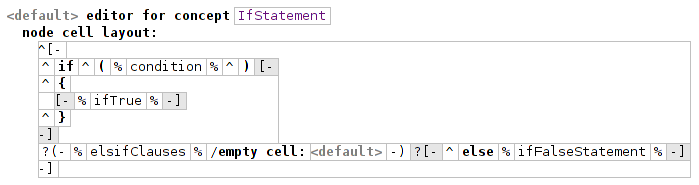
\includegraphics[scale=0.5]{./images/if_statement_editor_definition.png}
	\caption{"If statement" editor aspect definition}
	\label{fig:if_editor_definition}
\end{figure}

\JB{Nasledujici odstavec navrhuji odstranit}
\todo{From thesis.

The editor is a module dedicated/responsible for the definition of appearance of an AST node (concept).
JetBrains have developed a cellular system that allows placing node's (concept's) properties and children into different cells.
These cells then can be styled to user's liking.
There are many different types of cells, each behaving a little bit different towards its contents.
For example, MPS supports various horizontal and vertical lists, etc.
Extra cells can be added on top --- cells which just specify layout adjustments such as indentation and text color.
In Figure~\ref{fig:if_editor_definition}, you can see what a real editor definition might look like for the if statement of the Java language (as defined in MPS).
}

\paragraph{BaseLanguage}
\todo{Introduce the base language here.}
\JB{Odstavec prepsan}
In order to implement MPS itself and also to support the basic set of language-definition DSLs, BaseLanguage was developed in the early days of MPS. BaseLanguage is a clone of Java implemented using the MPS constructs. Although BaseLanguage is syntactically almost identical to Java, it is edited in a projectional editor, just like all languages in MPS. The DSLs that language authors use in order to define languages are generated into BaseLanguage. Similarly, all customer DSLs that are meant to be generated into Java choose BaseLanguage as their generation target and the conversion to textual Java will be handled by BaseLanguage without any further effort, since BaseLanguage has a TextGen aspect defined, which translates BaseLanguage code into textual Java sources.

\paragraph{TextGen.}
\JB{Odstavec upraven} The TextGen aspect defines how a certain AST node will be translated into text. The TextGen aspect is typically only needed for the bottom-line (base) languages. DSLs, on the other hand, need to define rules for model-to-model conversion (a generator), since these are rarely converted to text directly. After TextGen has generated textual sources from an AST, a compiler for the particular GPL gets invoke in order to compile the generate sources into binary code.
The TextGen definition follows a very straightforward pattern - each node outputs its textual representation into a textual buffer, calling TextGen of its children nodes at the right moments. MPS then calls this method for the root AST nodes of the given program.
TextGen aspect has to be defined (especially its more complex functionality) using the BaseLanguage.
Again, we included an example of the if statement (Figure~\ref{fig:if_statement_textgen}).

\begin{figure}[ht]
	\centering
	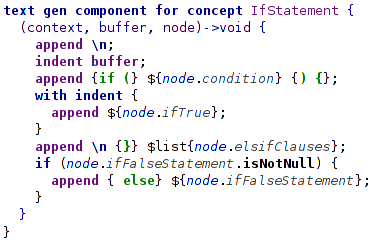
\includegraphics[scale=0.6]{./images/if_statement_textgen.png}
	\caption{"If statement" TextGen aspect definition}
	\label{fig:if_statement_textgen}
\end{figure}

\JB{Navrhuji odebrat}
\todo{From thesis.

After the program's AST is created using the projectional editor, there can be rules defined on how to generate code in plain text out of that tree.
This module is called "text gen".
These defined generators can target any language and platform.

\paragraph{Other aspects.}
MPS supports also other aspects, such as type checking, model transformations, static and data-flow code analysis, refactorings, language migrations, etc., but these are not important for our contribution. Moreover, the information needed for their automated generation is not available/contained inside a grammar file.

}

% TODO mozna zmenit nazev teto sekce
\subsection{Similar Projects}

We are aware of several projects that provide certain support for GPLs in the context of the MPS platform.
We will analyze existing related projects that are trying to accomplish similar goals, and then we will weigh advantages and disadvantages of these approaches.

Currently, there exists an almost full port of the Java language called BaseLanguage~\cite{ref:BaseLanguage} extended with some MPS specific features.
It was imported manually by JetBrains and it is still undergoing changes as Java itself is evolving.

Within the mbeddr project~\cite{ref:mbeddr}, the C language is also manually tailored for MPS.

Now/here we describe three similar projects (with similar goals) that we are aware of.
We focus on (consider) these three projects: PE4MPS, ANTLR{\_}MPS, and mps-metabnf.

\paragraph{PE4MPS.}
PE4MPS~\cite{ref:PE4MPS} is a project by Marco Lombardo that is trying to solve the same problem as we do.
It solves the lack of information about code layout in grammars by creating a new grammar notation called PE Grammars~\cite{ref:PE} (the PE abbreviation comes from projectional editing).
It has tw components: PE parser and PE4MPS plugin for MPS.
Their approach is to mimic an existing grammar notation called ANTLRv4~\cite{ANTLR4} and enrich its syntax with custom (their own) constructs.
These extensions tell (guide, hint) the parser what the AST node layout should look like.
Supported extensions (already implemented) include horizontal and vertical lists, and some indentation rules --- however, even these few features make the already not-so-simple syntax of ANTLR v4 much more complex.
The parser then uses this information when generating the projectional editor for am AST node.
Author of this approach/project described the PE syntax using the ANTLRv4 notation~\cite{ANTLR4reference} and then used the ANTLR toolset to automatically generate an ANTLRv4 parser for PE grammar files.
The PE parser reads any PE file and stores the language structure found inside to a custom representation of Java objects.

The PE4MPS plugin/project/tool is built on top of the PE parser.
This plugin uses the PE parser to build the PE file representation (the aforementioned tree-like structure of Java objects) and then creates AST nodes and their aspects inside MPS.
The extended syntax brought by PE describes the layout of each element, e.g. it tells the plugin that one set of child nodes should be displayed horizontally, another set should be vertical with each child on a separate line and with some indentation, and so on.

A limitation of the PE4MPS approach is that it, from what we understand, does not implement full ANTLR syntax.
This means that every grammar might need a non-trivial adjustment before its usage.
One of our goals is to enable import of as many languages out-of-the-box as possible and adopting the full specification.

\paragraph{ANTLR{\_}MPS.}
\PV{Tenhle projekt byl z tech tri nejmene uzitecny a podle me i nejmene funkcni, tak mozna by se dal v ramci zkracovani vypustit. V dalsim projektu je na nej reference, tak treba ji vyhodit.}
ANTLR{\_}MPS~\cite{ANTLR2MPS} is another project that is dealing with a similar problem.
The author of this project is Fabien Campagne.
The ANTLR{\_}MPS project also uses ANTLRv4 grammar notation~\cite{ANTLR4} and tries to import grammars inside MPS.
However, it does not try to generate the projectional editor at all (i.e., it does not deal with this problem), probably because it is in an early stage of development.

The way this import process of ANTLR{\_}MPS works is quite different from what we have seen in the PE4MPS project, and it is quite complex/complicated to use.
It works as follows. We give only a brief high-level overview and omit low-level technical details.
The author created a whole new ANTLRv4 MPS language, which is an MPS port of the grammar notations' syntax.
To import a language, the user utilizes this MPS ANTLR language.
The textual grammar is imported automatically into MPS taking the form of the MPS's ported grammar language (so that the textual grammar is converted into MPS nodes, that means an AST node is created for each grammar rule).
No child-parent relationships in the structure are generated by the tool --- all must be created manually by the user.
There are no editor nor TextGen aspects created neither.

\paragraph{mps-metabnf.}
\PV{Pridal jsem popis projektu}
% TODO - citace na https://github.com/DSLFoundry/mps-metabnf
The mps-metabnf project comes from the DSLFoundry group and also takes on grammar importing.
Even though it is in a very early stage of development, it holds some interesting ideas.
Similarly to ANTLR{\_}MPS, authors of mps-metabnf decided to create an MPS language describing the grammar.
When grammar is being imported into MPS, it is just transformed into the terms of this MPS language.
User is then able to adjust this grammar.
After this, a second step of the import process is needed, that generates the final MPS language out of this adjusted grammar definition.

The key takeaways from the mps-metabnf project are that the intermediate grammar MPS representation, when finished, will offer some powerful means of adjustment.
Using the projectional editor, the user can easily specify information about the code layout, export the target MPS language and, in case further adjustments are needed, come back to the grammar definition, fix any problems and regenerate the language.
The MPS language of the grammar definition can be easily extended with needed features (indenting, line breaks...), which is superior to our approach, because they can be represented using many visual means.

This approach also has some downsides.
Because MPS doesn't offer any tools that would allow easy transformation from the MPS grammar to the MPS language, the second step of the import process hasn't been implemented yet and will be probably very problematic.
Another downside might be the need for a double transformation implementation -- first one being the import of the text grammar to the MPS grammar definition.

From another point of view -- for each additional feature, that we decide to add to the grammar notation, we need to implement a corresponding transformation.
This subsequently leads to duplicating the projectional editor that is already present in MPS.
This means that there needs to be a line drawn between which features are added and which will be left for the user to add to the target language using MPS.


